\documentclass{ximera}


% using tikz for drawing graphs
\usetikzlibrary{arrows,positioning} 
\usetikzlibrary{arrows,shapes,backgrounds,through,shadows}
\usetikzlibrary{decorations.pathmorphing}
\usetikzlibrary{calc}
\tikzstyle{ugraph}=[line width=1.5pt]
\tikzstyle{cont}=[circle, draw,% a shading that is white at the top...
thick,minimum size=6mm,line width=1pt,>=stealth]  % continuous  node


\title{Algorithms}

\begin{document}
\begin{abstract}
The algorithms portion of the self-evaluation test for the University
of Leuven's Masters of Artificial Intelligence program.
\end{abstract}
\maketitle

% Question 19
% TODO (Behrouz) fix the algrithm so that it is shown in the webpage correctly
\begin{question}
Consider the algorithm below for: 
\begin{algorithm}%[Function(Array $A$)]
\begin{algorithmic}
  \FOR{$i = 1$ to $A$.length}
  \FOR{$j = 1$ to $A$.length--i}
  \IF{$A[i+1] < A[i]$}
  \STATE $temp = A[i]$
  \STATE $A[i] = A[i+1]$
  \STATE $A[i+1] = temp$
  \ENDIF
  \ENDFOR
  \ENDFOR
  \STATE output $A$
\end{algorithmic}
\end{algorithm}

% \begin{image}
% 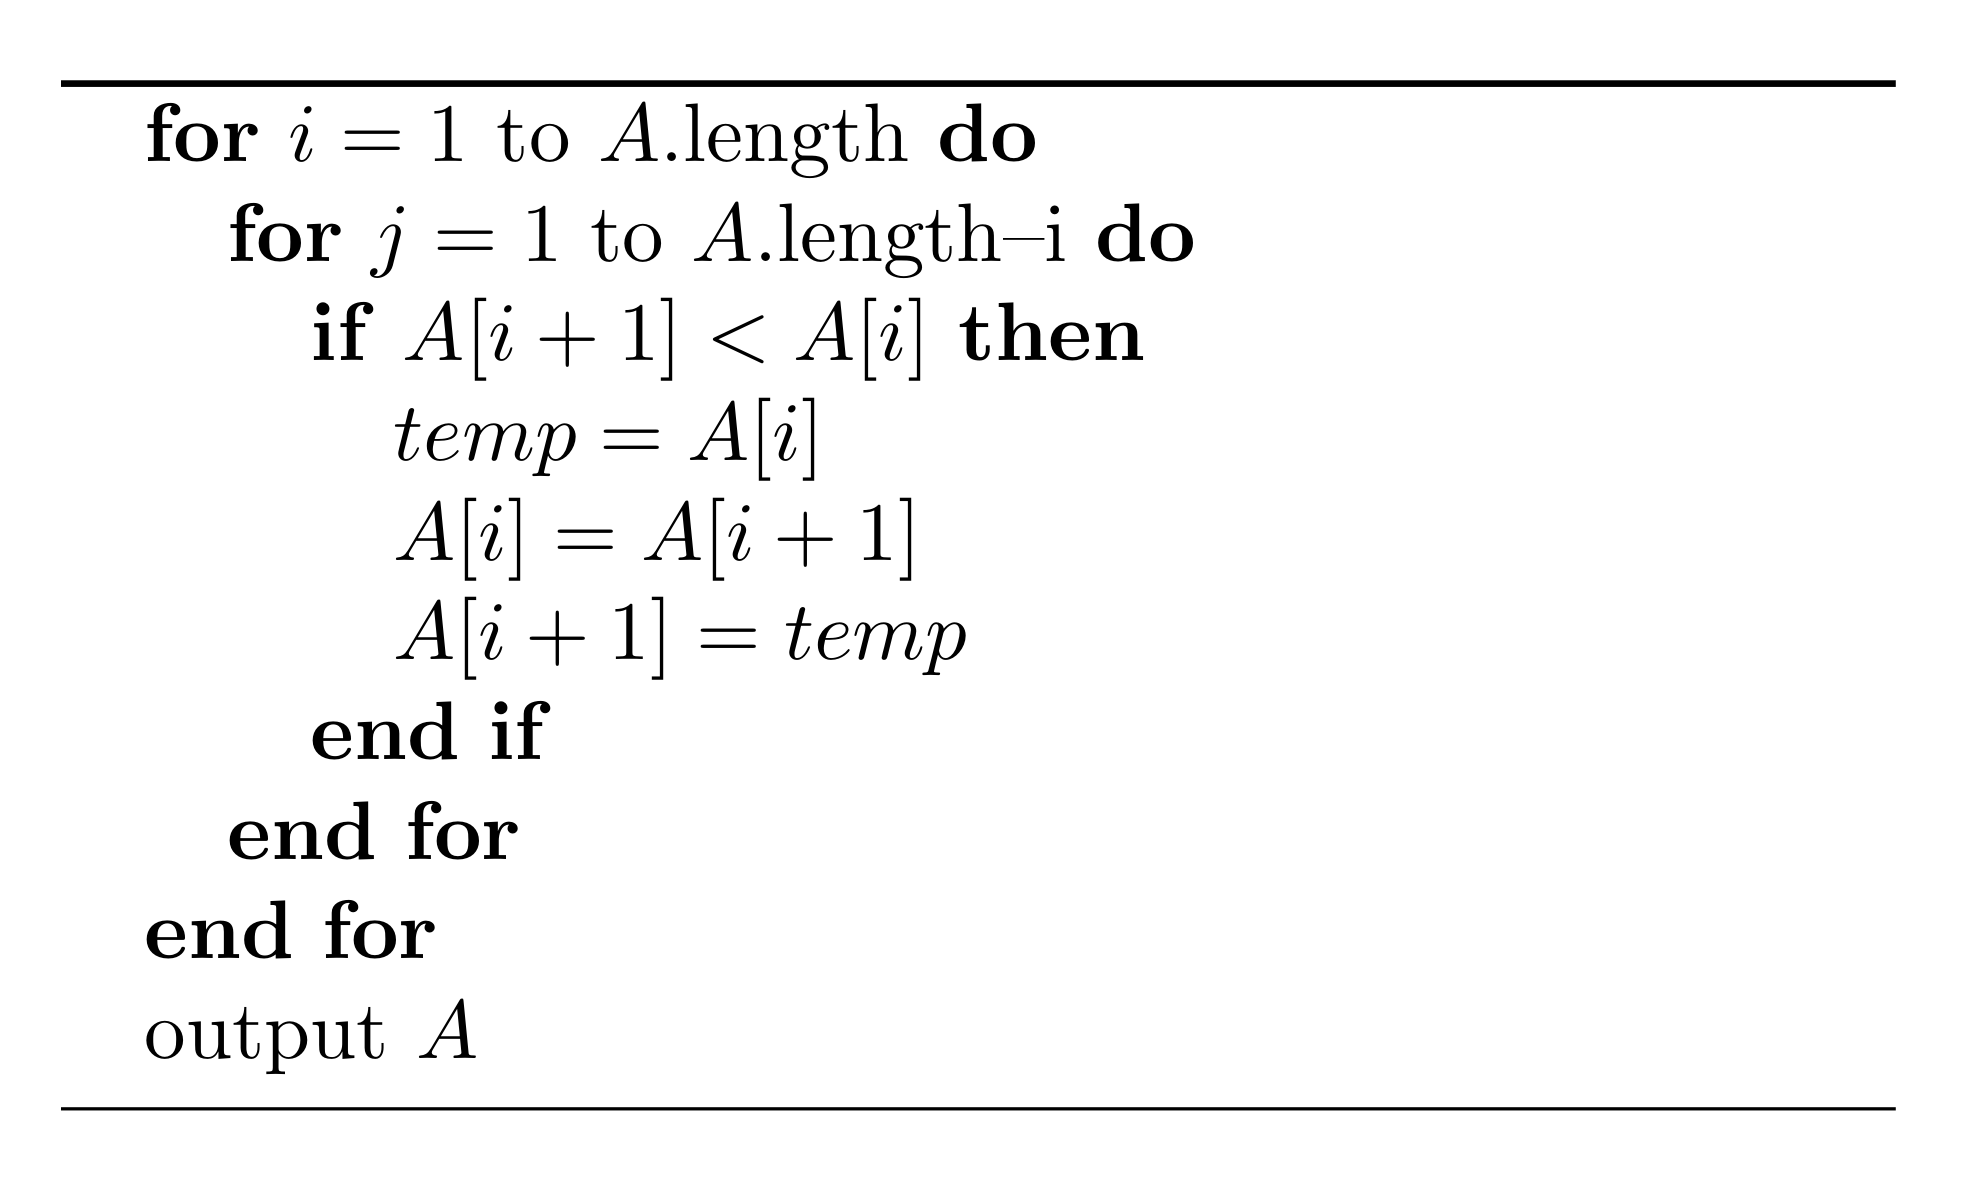
\includegraphics[width=0.6\textwidth]{algo.png}
% \end{image}


% part 1 of question
If the algorithm is invoked on the array $[ 5\quad 7\quad 3\quad 9]$ what is the output of the algorithm?
\begin{solution}
The output is 
\begin{matrix-answer}[name=M]
    correctMatrix = [['3','5','7','9']]
\end{matrix-answer}
\end{solution}

The output is:
$ [3 \quad 5 \quad 7 \quad 9] $

% part 2 of question
What does the algorithm do? 
% TODO (Behrouz) Verify if this is a correct implementation of free-response
\begin{free-response}
\end{free-response}
This algorithm sorts the input array using a technique called bubble sort.

% part 3 of question
Given an array with ten elements, how many comparisons (that is, $<$)
operations does the following piece of code perform?
\begin{solution}
There are \answer{45} comparisons.
\end{solution}  
The number of iterations of the inner loop starts with value 9 and
gradually decreases to 1. So the total number of comparisons is $ 9 +
8 + \ldots + 2 + 1 = 45$.

% part 4 of question
Can you generalize your answer such that it gives an upperbound on the
number of comparison operations for an array of length $n$?
\begin{solution}
\begin{hint}
Are you familiar with asymptotic analysis of algorithms (especially
the Big-$\Theta$ notation)?
\end{hint}
The smallest upper bound (expressed as a function of $n$) is
\answer{$n^2$}.
\end{solution}
For an array of length $n$, the number of iterations of inner loop
starts with value $n-1$ and gradually decreases to 1. So the total
number of iterations would be $(n-1) + (n-2) + \ldots + 1 =
\frac{n(n-1)}{2}$. This indicates that the running time of this
algorithm is of $\Theta(n^2)$.
\end{question}

% Question 21
\begin{question}
What is the maximal number of leaves that a sorted binary tree with depth $4$ can possess?
\begin{solution}
The answer is \answer{16}.
\end{solution}
The maximal number of nodes at depth-level $d$ of a binary tree is $2^d$. So the answer to this question is $2^4 = 16$. 
\end{question}

% Question 22
\begin{question}
Order the following functions according to their growth-rate (use the theory of big-Oh notation). Put the slower growing functions first.
\[
n^7, 8n!, 5 \log_2 n,~ 3n, 2^n, ~ 7.5 n\log_2 n, ~ 6 n^2
\]
\begin{solution}
Present your answer as a row vector of numbers in the following way: The first entry of vector is the position of the first element of the original (unordered) list in the new (ordered) list, the second entry is the position of the second element of original list in the new list, and so on. The positions in a list start at 1.

\begin{matrix-answer}[name=M]
%    correctMatrix = [['5\log_2^n','3n','7.5n\log_2{n}','6n^2','n^7','2^n','8n!']]
     correctMatrix = [['5','7','1','2','6','3','4']]
\end{matrix-answer}
\end{solution}

This is the list of functions ordered according to their growth-rate:
\begin{equation*}
5 \log_2^n \prec 3n \prec 7.5 n \log_2{n} \prec 6n^2 \prec n^7 \prec 2^n \prec 8n!
\end{equation*}
\end{question}

\end{document}
